\documentclass[ngerman, 12pt,a4paper]{article}

\usepackage[ngerman]{babel}

% formatting
\usepackage[left=3cm, right=3cm, top=3cm, bottom=3cm]{geometry}

% package for nonstandard letters (umlauts etc)
\usepackage[utf8]{inputenc} 

%% Mathematics
\usepackage{amsmath,amsfonts, latexsym, amssymb}

%% Graphics
\usepackage{graphicx}
\usepackage{subfigure}

%% Code
\usepackage{listings} 

%% For nice tables
\usepackage{booktabs}

%% Line spacing
\renewcommand{\baselinestretch}{1.5}

%% Bibliography
\usepackage{cite}

%% to avoid messy linebreaks
\sloppy

\begin{document}


\begin{center}
\thispagestyle{empty}

{\huge Projekt NoSQL}\\[1.5cm]


\large
\begin{tabular}{rl}
\hline
Author:  &Lukas Lieb\\ 
				& Daniel Schmid \\
				& Matthias Eiholzer \\

E-Mail: & lukas.lieb@stud.hslu.ch \\
				& daniel.schmid@stud.hslu.ch \\
				& matthias.eiholzer@stud.hslu.ch\\
Erstellungsdatum: & \today\\
\hline
\end{tabular}
\end{center}



%%%%%%%%%%%%%%%%%Abstract%%%%%%%%%%%%%%%%%%%
\begin{abstract}
\LaTeX  
\end{abstract}
\newpage
%%%%%%%%%%%%%%End: Abstract%%%%%%%%%%%%%%%%


%%%%%%%%%%Table of contents %%%%%%%%%%%%%%%
\tableofcontents
\newpage
%%%%%%%%End: Table of contents %%%%%%%%%%%%

\listoffigures
\newpage
%\listoftables
%\newpage


\section{Einführung}
Im Modul DMG wurde zu Übungszwecken zu relationalen Datenbanken die Uni-DB 
verwendet. Das dabei verwendete Entity-Relation Diagramm ist in Abbildung
\ref{fig:uni-db} ersichtlich.
\begin{figure}[htbp] 
  \centering
     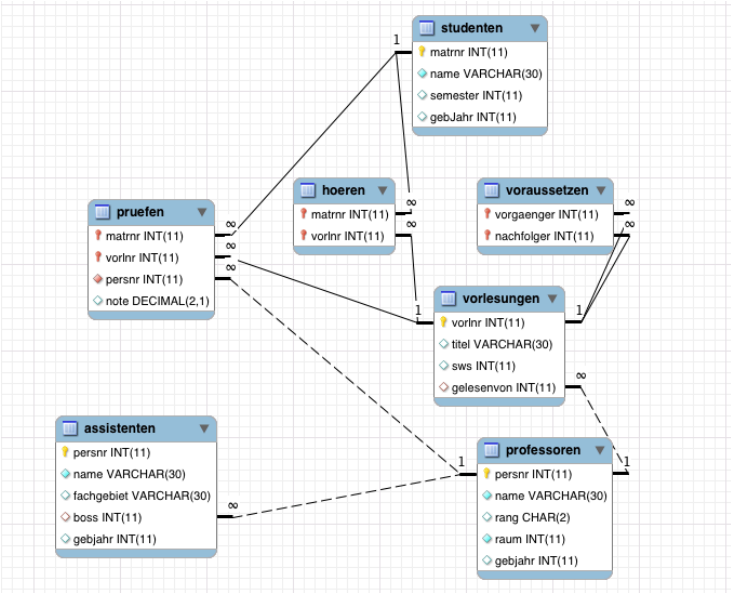
\includegraphics[width=1\textwidth]{./pictures/SQL-DB_ER_Diagramm_UNI-DB.png}
  \caption{ER-Diagramm zur Uni-DB \cite{Kaufmann2016_S1}}
  \label{fig:uni-db}
\end{figure}
 Um mit den NoSQL Datenbanken Erfahrung zu sammeln, wird dieses Schema in die NoSQL Datenbank MongoDB überführt.
Die MongoDB ist eine dokumentorientierte Datenbank und  wird aus folgenden
Gründen für dieses Projekt verwendet:
\begin{itemize}
  \item Geeignet um unser Problem zu lösen.
  \item Wird in der Praxis eingesetzt
  \item Gute Dokumentation
  \item Kostenfrei
  \item Untstützung durch Forenuser
  \item Erste Erfahrung vorhanden
\end{itemize}
Die Aufgabe besteht darin, ein vorgegeben SQL-Query so in MongoDB Operationen
abzubilden, dass die MonogDB Abfrage das selbe Resultat ergibt wie das folgende 
SQL-Query
\begin{lstlisting}
select ProfessorName, AnzahlStudenten, SummeSWS 
from ( 
	select p.Name as ProfessorName, count(s.MatrNr) 
	as AnzahlStudenten 
		from Professoren p 
		join Vorlesungen v on v.gelesenVon = p.PersNr
		join hoeren h on h.VorlNr = v.VorlNr 
		join Studenten s on s.MatrNr = h.MatrNr 
		group by p.Name 
	) A 
join 
( 
	select p.Name as ProfessorName,  sum(SWS) 
	as summeSWS 
	from Professoren p 
	join Vorlesungen v on v.gelesenVon = p.PersNr 
	group by p.Name 
) B using(ProfessorName)
\end{lstlisting}

 \section{Datenmanagement}
Zwei Aktoren wirken auf die Datenbank ein. Einerseits der Benutzer, welcher die
Informationen abfragen kann. Andererseits der DB-Administrator, welcher die
Daten abfragen, aber auch verändern und neue hinzufügen kann. Diese
Anwenungsfälle sind in der Abbildung \ref{fig:usecase} abgebildet.
%\begin{figure}[htbp]
%  \centering
%     
\includegraphics[width=1\textwidth]{./pictures/todo.jpg}
%  \caption{Visualisierung des Anwenungsfalls}
%  \label{fig:usecase}
%\end{figure}


Welche Daten werden integriert migriert
 und wie werden sie 
aufbereitet?
Wie interagiert der Benutzer mit der Datenbank?

Der Benutzer hat die Möglichkeit, über ein GUI Daten auf der Datenbank abzufragen. Dies beinhaltet lediglich die Abfrage der Professoren und wie viele SWS Punkte die entsprechenden Professoren unterrichten.

\section{Datenmodellierung}
\label{kap:ERDiagramm}
MongoDB ist eine Dokument orientierte Datenbank. Dabei werden die Daten in JSON
ähnlichen Dokumenten verwaltet. Um das Entity-Relations Schema in die MongoDB
abbilden zu können, muss das Schema umgeformt werden. Dies ist auch bei
relationalen Datenbanken der Fall. In Abbildung \ref{fig:uni-db} ist das
ER-Schema der uni-DB abgebildet. Dies ist die Ausgangslage für unser Projekt.
MongoDB ist eine dokumentorientierte Datenbank. Dabei werden die Daten in Dokumenten verwaltet, die im JSON Format gespeichert werden. Das bedeutet, dass die Daten nicht relational
verwaltet werden. So kann zum Beispiel ein Tupel einer relationalen Datenbank
als Dokument in der dokumentorientierten Datenbank abgebildet werden. Die
Attribute und die dazugehörigen Werte werden dabei in Schlüssel-Wert Paare
abgebildet. 
\\\\
Unserem Projekt liegt das ER-Schema aus Abbildung \ref{fig:uni-db}
zugrunde.
Da MongoDB eine NoSQL und keine relationale Datenbank ist, kann das ER-Schema nicht direkt
in dieser Form in der Datenbank abgebildet werden. 

\begin{figure}[h] 
	\centering
		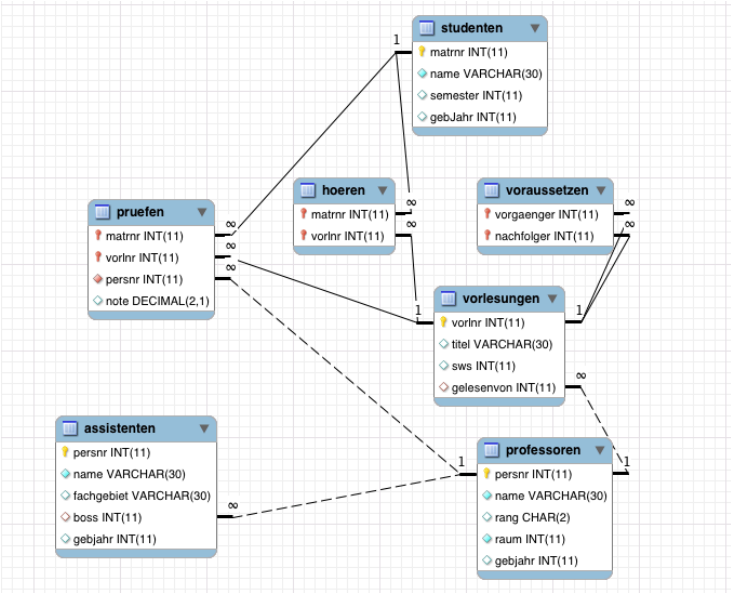
\includegraphics[width=1\textwidth]{./pictures/SQL-DB_ER_Diagramm_UNI-DB.png}
	\caption{ER-Diagramm zur Uni-DB \cite{Kaufmann2016}}
	\label{fig:uni-db}
\end{figure}

Das Schema der NoSQL Datenbank sieht wie folgt aus:
\begin{figure}[h] 
	\centering
		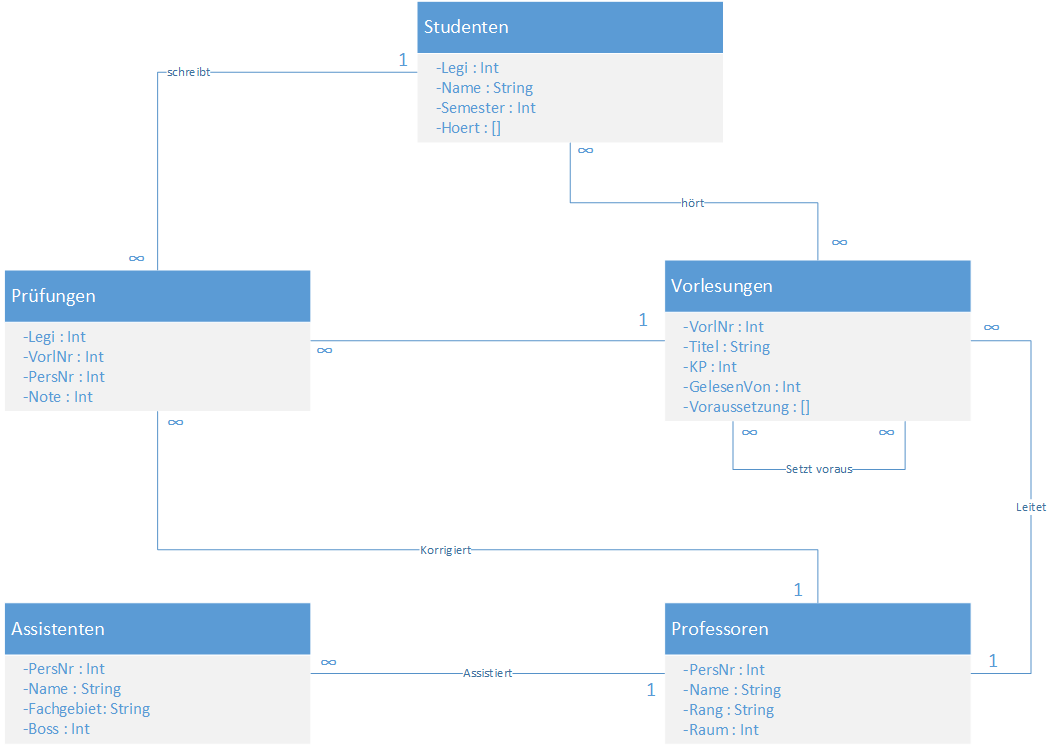
\includegraphics[width=1\textwidth]{./pictures/NoSQL-DB_ER_Diagramm_UNI-DB.png}
	\caption{ER-Diagramm zur Uni-DB}
	\label{fig:uni-db}
\end{figure}
Eine Collection der MongoDB entspricht der Tabelle in relationalen Datenbanken.
Das Dokument ist das Gegenstück zum Tupel. Die Attribute und die dazugehörigen
Werte werden in der MongoDB als Schlüssel-Wert Paare gespeichert.
Beziehungen werden in RDBMS als Fremdschlüssel abgebildet. In MongoDB 
können Relationen in Form von Werten eines bestimmten Keys gespeichert werden.
Komplex-Komplexe Beziehungen werden in RDBMS in eigene
Tabellen ausgelagert. Daraus entstehen dann zwei Einfach-Komplexe
Beziehungen. \\
Wie bereits erwähnt, muss das ER-Schema auch für die MongoDB umgeformt werden.
Starke Entitäten werden als Collections abgebildet, schwache Entitäten werden 
als Unterteil in das dazugehörige Dokument eingebettet.
Das Schema nach der Umformung ist in der Abbildung \ref{fig:uni-dbNoSQL}
ersichtlich.
\begin{figure}[h] 
	\centering
		
\includegraphics[width=1\textwidth]{./pictures/todo.jpg}
	\caption{MongoDB Schema zur Uni-DB }
	\label{fig:uni-dbNoSQL}
\end{figure}
Eine Komposition bedeutet, dass eine schwache Entität als Unterteil abgebildet
wird. Eine Aggregation bedeutet, dass starke Entität  als Referenz abgebildet
wird. In MongoDB wird die ID des Referenzierten Dokuments als Wert gepsiechert.
\\
Der folgenden JSON-Code zeigt ein Beispiel wie eine starke Entität
in MognoDB abgespeichert wird. Das Code-Beispiel zeigt das Dokument eines
Studenten. Die Vorlesungen, welcher dieser Student hört, werden im Werte Array
des Schlüssels Hören abgespeichert. Die Werte entsprechen dabei der ID der
Vorlesung.
 \begin{figure} [h]
	\begin{verbatim}
	{
		"Legi": 25403,
		"Name" : "Jonas",
		"Semester" : 12,
		"Hören" : [5032, 1910],
	}
	\end{verbatim}
	\label{cod:vorlesung}
\end{figure}




 \section{Datenbanksprachen}

 \section{Konsistenzsicherung}
 Bei relationalen Datenbanken bietet die Datenbank Mechanismen zur
 Konsistenzsicherung an. Dies wird durch verschiedene Eigenschaften im RDBMS
 erreicht. Jeder Tabelle liegt ein Schema zu Grunde. In diesem wird definiert,
 wie die Daten strukturiert sein müssen. Zum Beispiel wird festgelegt, welches
 der Primärschlüssel ist, ob Felder ``null'' sein dürfen oder ob Tupel gelöscht
 werden dürfen wenn noch Referenzen darauf zeigen.
 \\\\
 MongoDB ist Schema frei. Das bedeutet, dass sich je zwei Dokumente in einer
 Sammlung  komplett in ihrer Struktur voneinander unterscheiden können.
 Des Weiteren garantiert MongoDB keine Integrität der Referenzen. Dieser Umstand
 wird klar, wenn verglichen wird, welchen Regeln relationale Datenbanken und
 die MognoDB unterliegen.
 \\\\
 \noindent
 RDBMS unterliegen den ACID Regeln:
 \begin{itemize}
   \item Atomar: Die gesamte Transaktion wird ausgeführt oder die Transaktion
   wird rückgängig gemacht.
   \item Consistent: Nach jeder Transaktion muss die Datenbank widerspruchsfrei
   sein.
   \item Isolatet: Bei einer Transaktion dürfen keine Seiteneffekte
   auftreten. Dies garantiert, dass ein Mehrbenutzerbetrieb möglich ist.
   \item Dauerhaft: Die Daten werden sicher gespeichert, auch bei
   Systemabstürzen. Bei einem Systemabsturz wird ein Recovery durchgeführt, so 
   dass danach die Datenbank wieder in einem konsistenten Zustand ist.
 \end{itemize}
 Die in unserem Projekt eingesetzte MongoDB unterliegt den BASE Regeln.
 \begin{itemize}
   \item Basically Available: Die Datenbank sollte meistens laufen.
   \item Eventually Consistent: Die Konsistenz der Daten wird nicht unmittelbar
   nach der Operation gewährleistet. Sie kann verzögert eintreten.
\end{itemize}
\noindent
Da MongoDB keine Transaktionen (eine Folge von Operationen, die Atomar
ausgeführt werden) unterstützt, muss diese Funktionalität auf der
Anwendungsebene implementiert werden. Dies ist beim Einsatz eines RDBMS nicht
notwendig, da dieses Transaktionen unterstützt. Im Falle dieses Projektes werden keine
Transaktionen verwendet, da nur lesend auf die Daten zugegriffen wird.
Da keine Daten geändert oder hinzugefügt/entfernt werden,
kann die Datenbank durch Operationen nicht in einen inkonsistenten Zustand
überführt werden. Deswegen kann auch parallel auf die Daten zugegriffen
werden, ohne die Konsistenz zu verlieren. Sollen zu einem späteren Zeitpunkt zur
Laufzeit der Anwendung Daten geändert oder hinzugefügt/entfernt werden,
 so muss eine Konsistenzsicherung auf der Anwendungsebene  implementiert werden.


 

		
 
 \section{Systemarchitektur}
 MongoDB besteht aus drei verschiedenen Servern. Den Routern, Config Servern und
 den Replica Sets. Jeder dieser drei Servertypen hat eine bestimmte Aufgabe.
 Der Client sendet seine Operation an den Router. Der Router wiederum leitet
 die Operation an die zuständigen Replica Sets weiter. Die Replica Sets wiederum 
 speichern die zu verarbeitenden Dokumente. Damit der Router weiss, an welche
 Replica Sets er die Anfrage weiterleiten muss, stellt er wiederum eine Anfrage
 an die Config Server. Diese Antworten entsprechend. Die Config Server enthalten 
 also die Metadaten über die Dokumentenverteilung in den Replica Sets.
 In der Abbildung \ref{fig:archmong} ist die Architektur von MongoDB
 visualisiert.
\begin{figure}[htbp]
	\centering
    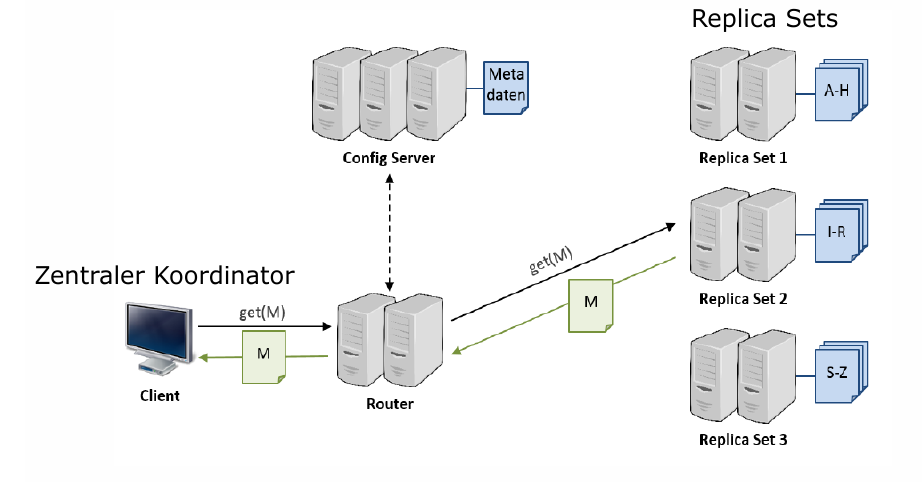
\includegraphics[width=1\textwidth]{./pictures/Architektur_MongoDB.png}
  \caption{Architektur von MongoDB. \citet{Kaufmann2016_DB}}
  \label{fig:archmong}
\end{figure}
 In der in diesem Projekt eingesetzte MongoDB Instanz, laufen alle drei Server
 auf demselben physischen Rechner. Dies wurde so gewählt, da die Sammlungen an
 Dokumenten klein ist. Des weiteren wird auch nur sporadisch auf die Daten
 zugegriffen. Sollte sich in Zukunft einer dieser Parameter ändern, kann darüber
 nachgedacht werden, die Server auf verschiedene physische Server zu
 verteilen. Dies hätte auch den weiteren Vorteil, dass parallel auf die
 Dokumente zugegriffen werden kann. Ist die Replica Set 1 mit der Verarbeitung
 einer Anfrage beschäftigt, kann gleichzeitig die Replica Set 2 die nächste
 Anfrage bearbeiten, sofern es sich bei der Anfrage um die in ihr gespeicherten
 Dokumente handelt. \\
 In RDBMS liegen die Tabellen in normalisierter Form vor. Daten die nicht
 funktional vom Primärschlüssel abhängen, werden als Fremdschlüssel
 referenziert. Die Referenzierung macht es schwierig, die Tabelle, in
 welcher das referenzierte Tupel abgelegt ist, auf einen anderen Server
 auszulagern. Denn bei jedem Zugriff auf die ausgelagerte Tabelle, wird die
 Abfrage der Daten verlangsamt, da zwischen den beiden Servern Kommunikation
 stattfindet. Dieses Problem hat MongoDB nicht, da die Daten nicht normalisiert
 vorliegen müssen. Bei MongoDB dürfen die bei RDBMS referenzierten Tupel als
 Aggretationen in die Dokumente umgesetzt werden. Dies vermindert die Anzahl der
 Referenzierungen und ermöglicht es damit, dass eine horizontale Skalierung
 einfacher zu bewerkstelligen ist, als bei einer relationalen Datenbank. Dies
 führt auch Nachteile mit sich. Jedes mal wenn ein referenziertes
 Tupel als Aggregation in ein Dokument gespeichert wird, erhöht sich die
 Datenmenge. Des weiteren bedeutet es mehr Aufwand, ein solches aggregiertes
 Tupel zu ändern, da die Änderung bei allen Dokumenten gemacht werden muss, bei denen
 das referenzierte Tupel als Unterteil gespeichert wird. Dies im Gegensatz zur
 relationalen Datenbank. Bei dieser muss die Änderung nur an einem Ort
 stattfinden. MongoDB kennt keine Funktionlität zum Auflösen von Referenzen.
 Diese muss jeweils in der Applikation implementiert werden. \\
 Da wie bereits erwähnt, alle Server auf einem physischen Rechner
 laufen, ist die Datenbank bei einem Systemausfall nicht mehr erreichbar.
Bei einem Festplattenausfall kann es sogar passieren, dass die komplette
Datenbank verloren geht, da es in der Replica Set nur einen Server gibt, und
somit ein weiter Server fehlt, der ein Replikat der Datenbank enthält.
 

\section{Schlussfolgerungen}
Nach dem Entscheid über die NoSQL Datenbank konnten wir erfolgreich eine Instanz
von MongoDB aufsetzten. Zudem war es uns möglich per API der Datenbank über das
Konsolenfenster Daten hinzuzufügen, zu ändern oder löschen. Die
Robomongo\cite{Robomongo2016} Applikation ermöglichte es uns die Änderungen auf
einfache Art zu kontrollieren. Nach dem Einarbeiten in die Syntax des Mongo-Java Treibers war es uns auch möglich Änderungen an der Datenbank von einem Javaprogramm aus vorzunehmen.
\\\\
Bei diesem Projekt ist uns klar geworden wie sehr sich NoSQL- von SQL-Datenbanken unterscheiden. Wir haben zwar schon vermehrt in der Theorie davon erfahren, allerdings ist es etwas ganz anderes dies in der Praxis zu erleben. Zudem ist es bei NoSQL Datenbanken viel wichtiger die Applikation sauber aufzubauen, da einem die API der Datenbank viel weniger Funktionen zur Verfügung stellt als beispielsweise bei einer SQL Abfragesprache. 
\\\\
MongoDB ist grundsätzlich sehr einfach installiert und es läuft sehr stabil. Auch die gebotene Abfragesprache ist nach einer kurzen Zeit sehr einfach und intuitiv. Grundsätzlich ist MongoDB im CP Bereich also Consistency und Partition-Tolerance angesiedelt. Die Möglichkeit auf Kosten der Consistency die Availability zu erhöhen macht sie zusätzlich für weitere Anwendungsgruppen sehr attraktiv. Die Datenbank verfügt über eine grosse Community, durch welche reichlich Hilfe bei Problemen zur Verfügung steht. Ausserdem ist sie auch sehr gut Dokumentiert.
\\\\
Sie verfügt aber auch über gewisse Nachteile. So ist sie zum Beispiel nicht für alle Anwendungstypen einer NoSQL Datenbank ausgestattet. Zudem ist sie nicht abgesichert wenn mehrere Benutzer gleichzeitig auf der Datenbank Änderungen vornehmen. Bei gewissen Szenarien ist es zudem von Vorteil wenn sauber referenziert werden kann. Dies ist bei MongoDB und auch allgemein bei NoSQL Datenbanken nicht immer ideal.
\\\\
Allgemein werden SQL Datenbanken häufiger in System verwenden, in denen die Konsistenz sehr hoch sein muss, wie zum Beispiel bei Banken oder auch Versicherungen. NoSQL Datenbanken werden dabei eher bei Datenmenge wie BigData oder auch bei grösseren WebServices eingesetzt. MongoDB speziell sollte bei Systemen zum Einsatz kommen, die eine hohe Daten Übereinstimmung bei den einzelnen Nodes und eine gute Ausfallsicherheit voraussetzen.



 %%%%%%%%%%%Bibliography%%%%%%%%%%%
\newpage
% to have more compact display of references
\bibliographystyle{plain}
% enter the name of your jabref file
\bibliography{myreferences}
\newpage

%%%%%%%%%%%Anhang%%%%%%%%%%%%%
%\begin{appendix}
\section{Anhang}

\end{appendix}



\end{document}
